% !TeX spellcheck = cs_CZ
% options:
% thesis=B bachelor's thesis
% thesis=M master's thesis
% czech thesis in Czech language
% slovak thesis in Slovak language
% english thesis in English language
% hidelinks remove colour boxes around hyperlinks
\RequirePackage{color}
\definecolor{gr1}{RGB}{0,153,51}
\documentclass[thesis=M,czech]{FITthesis}[2012/06/26]


\usepackage[utf8]{inputenc} % LaTeX source encoded as UTF-8

\usepackage{graphicx} %graphics files inclusion
\usepackage{amsmath} %advanced maths
\usepackage{amssymb} %additional math symbols
\usepackage{rotating}

\usepackage{dirtree} %directory tree visualisation
% % list of acronyms
% \usepackage[acronym,nonumberlist,toc,numberedsection=autolabel]{glossaries}
% \iflanguage{czech}{\renewcommand*{\acronymname}{Seznam pou{\v z}it{\' y}ch zkratek}}{}
% \makeglossaries
 

\newcommand{\tg}{\mathop{\mathrm{tg}}} %cesky tangens
\newcommand{\cotg}{\mathop{\mathrm{cotg}}} %cesky cotangens

% % % % % % % % % % % % % % % % % % % % % % % % % % % % % % 
% ODTUD DAL VSE ZMENTE
% % % % % % % % % % % % % % % % % % % % % % % % % % % % % % 

\department{Katedra geomatiky     }
\acknowledgements{Studijní program Geodézie a kartografie}

\title{Kartografická vizualizace vývoje území v údolí řeky Otavy v okolí Strakonic}
\authorGN{Petra} %(křestní) jméno (jména) autora
\authorFN{Pasovská} %příjmení autora
\authorWithDegrees{Bc. Petra Pasovská} %jméno autora včetně současných akademických titulů
\supervisor{Ing. Tomáš Janata, Ph.D.}
\acknowledgements{Děkuji Ing. Tomáši Janatovi, Ph.D., za odborné vedení práce a cenné rady, které mi pomohly tuto práci zkompletovat. Velké díky také patří mé rodině a přátelům, kteří mi byli po dobu zpracování velkou oporou. Ráda bych také poděkovala panu Ladislavu Höllovi, který mi velmi pomohl se sběrem historických fotografií použitých v této práci a pracovníkům Stavebního úřadu ve Strakonicích za zapůjčení stavebních plánů Strakonického hradu.}
\abstractCS{Cílem této práce je vizualizace údolí řeky Otavy ve vybraném zájmovém území. Podstatou práce je zpracování kartografických podkladů pro různé časové hladiny. Výsledné zpracování dat je doplněno o generalizovaný 3D model Strakonického hradu. Součástí práce je také sběr historických fotografií zachycujících řeku Otavu a jejich porovnání se současným stavem. Okolí řeky je následně doplněno o objekty vytvořené konceptuálním modelováním v programu CityEngine. Na základě zpracování kartografických podkladů je  možné porovnat změnu využití půdy a říčního koryta. (tady to ještě poupravit ten konec, nějak pěkně vymyslet účel práce) }
\abstractEN{The aim of this work is visualize the Otava River valley in the selected area of interest. The essence of this thesis is the processing of cartographic materials for various time periods. The result is complemented by a generalized 3D model of Strakonice Castle. The thesis also includes the collection of historical photographs depicting the Otava River and their comparison with the current state. The surroundings of the river are then supplemented with objects created by conceptual modeling in the CityEngine program. }
\placeForDeclarationOfAuthenticity{V~Praze}
\declarationOfAuthenticityOption{1} %volba Prohlášení (číslo 1-6)
\keywordsCS{Otava, řeka, údolí, Strakonice, georeferencování, vektorizace, 3D model, ArcGIS, CityEngine, Sketchup \newpage}
\keywordsEN{Otava, river, valley, Strakonice, georeferencing, vectorization, 3D model, ArcGIS, CityEngine, Sketchup}

\begin{document}

% \newacronym{CVUT}{{\v C}VUT}{{\v C}esk{\' e} vysok{\' e} u{\v c}en{\' i} technick{\' e} v Praze}
% \newacronym{FSv}{FSv}{Fakulta stavebn{\' i}}

\begin{introduction}
Voda, nejdůležitější složka na Zemi. Zaujímá klíčové postavení nejen v přírodě, ale i v činnosti člověka. Přesto, že má voda schopnost se neustále obnovovat, její zásoby každým rokem klesají. Voda je nepostradatelnou součástí našich životů. Je nepostradatelným zdrojem pitné vody, využívá se pro zavlažování či v energetice. 

Pro zpracování bylo vybráno území v jižních Čechách poblíž města Strakonice, nazývané též střední Pootaví, kde díky velmi suchým létům začínají vysychat studny a některé domácnosti se díky tomu mohou ocitnout zcela bez vody. Kontrastem k těmto suchým obdobím jsou často zvýšené hladiny řeky Otavy, a to zejména na jaře při tání sněhové pokrývky na Šumavě a v srpnu, kdy je často velmi vydatný déšť, který nedokáže půda zcela pojmout.

V roce 2002 byla jedna z nejničivějších povodní na Otavě, která poškodila mnoho měst. Následkem toho vznikla nová protipovodňová opatření a města se začala připravovat na možnost, že by takto velká voda opět přišla. V této práci bude zkoumána změna toku a říčního koryta Otavy v různých časových hladinách. Na změnu říčního koryta má vliv i využití okolní půdy. Z tohoto důvodu byly vytvořeny hlavní kategorie využití půdy a následně vypočítán koeficient ekologické stability. 

Pro zhodnocení a vizualizaci údolí řeky Otavy bylo použito několik historických kartografických děl. Nejstarší podklady jsou Císařské povinné otisky stabilního katastru (1826-1843). (SEPSAT DALŠÍ KARTOGRAFICKÉ PODKLADY ZE KTERÝCH SE VYCHÁZELO). Neodmyslitelným symbolem řeky Otavy je Strakonický hrad, který vznikl na soutoku Otavy a Volyňky v 1. polovině 13. století. Z důvodu významnosti této stavby byl vytvořen generalizovaný 3D model hradu, který vizuálně doplní vytvořený model řeky. 

V rámci diplomové práce byl proveden také sběr historických fotografií. Pro doplnění práce byly použity nejen historické fotografie zachycující řeku Otavu, ale také fotografie Strakonického hradu. 

Diplomová práce je rozdělena na čtyři hlavní části. Začátek práce poskytuje seznámení s řekou Otavou z hydrologického, historického i kulturního hlediska. Ve druhé části jsou blíže popsána použitá data. Následně je konkrétně popsán způsob zpracování dat a metody, které byly v rámci diplomové práce použity. Závěr je věnován prezentování výsledků na webové stránce, která byla vytvořena v jazyce (NO PROSTĚ TADY SE ROZEPSAT AŽ SE ROZMYSLÍM JAK TU STRÁNKU NAPSAT)


\end{introduction}

\chapter{Rešerše literatury}
Tato práce se zaměřuje na tři hlavní témata - hydrologii, kartografii a modelování. Všechna témata jsou v dnešní době aktuální a existuje k nim mnoho publikací.

Knih o hydrologii byla publikována celá řada. Vzhledem k tomu, že na mnoha vysokých školách je hydrologie vyučována, vycházela jsem v této práci především ze studijních materiálů, a to zejména ze studijních materiálů VŠCHT a Univerzity Karlovy. Pro výklad termínů vztahujícím se k řekám byl použit Meteorologický slovník \cite{meteo} vytvořený Českou meteorologickou společností (ČMeS), který je dostupný na internetu zdarma. Některé definice byly čerpány také z knihy Ladislava Slavíka a Martina Nerudy Voda v krajině \cite{definiceHydro}. 

Pro zhodnocení řeky jako takové nejvíce posloužila kniha Základy fyzické geografie \cite{FGkniha}. Hydrologickou analýzou se ve velké míře zabývají na již zmíněné Univerzitě Karlově, kde byl vytvořen návod na cvičení od Miroslava Šobra \cite{UK}. Významnou publikací je také studijní materiál Hydrologie a hydropedologie od autorek Dany Pokorné a Jany Zábranské \cite{hydrovscht}. 

Kartografií zabývající se publikace jsou opět převážně studijní materiály. Pro vizualizaci zájmové oblasti byly využity Císařské povinné otisky stabilního katastru. O vzniku a vlastnostech (detailech?) těchto map se lze dočíst v publikaci od Růženy Zimové a Bohuslava Veverky Topografická a tematická kartografie \cite{topo_skripta}. Tématu mapování se také věnuje profesor František Hromádka, který s kolektivem autorů publikoval učební text Mapování \cite{mapovani_brno}.

Zmíněné historické podklady bylo nutné zgeoreferencovat. Popis transformací a zpracování historických děl je kvalitně obsaženo v díle Jiřího Cajthamla Analýza starých map v digitálním prostředí na příkladu Műllerových map Čech a Moravy\cite{transformace}. Autor se v tomto díle mimo transformace věnuje také popisu starých map našeho území a prezentaci vytvořených digitálních map.

Pro vizualizaci okolí řeky Otavy byly vytvářeny dílčí tematické mapy. Při tvorbě map je nutné dodržet stanovená kartografická pravidla. V této práci byla hlavním literárním zdrojem těchto pravidel díla od Růženy Zimové a Bohuslava Veverky Topografická a tematická kartografie \cite{topo_skripta}, učební text od Jaroslava Hybáška Topografická a tematická kartografie - učební texty \cite{tematicka_brno}, publikace Vybrané okruhy geografické kartografie od Jana D. Bláhy \cite{kartoblaha} a kniha Metody tematické kartografie - Vizualizace prostorových jevů od Víta Voženílka \cite{mapyolomouc}.

V rámci práce byly zkoumány možnosti 3D modelování objektů. Tomuto tématu se věnují především práce publikované v zahraničí, nejčastěji odborné články. Za zmínku jistě stojí článek publikovaný v časopise Minjiangské univerzity v roce 2016 \cite{cina}. Autoři v tomto článku popisují využití 3D modelování v územním plánování vytvořené v prostředí GIS ve městě Fuzhou. Na téma 3D modelování v prostředí GIS vyšel také článek v časopise International Journal of Risk Assessment and Management \cite{clanek_flood}. Autoři v tomto článku analyzovali, vizualizovali a simulovali povodňová rizika poblíž řeky Qu'Appelle v jižním Saskatchewanu. 

Na téma 3D modelování existuje mnoho zahraničních knih. Převážně se však týkají modelování z architektonického hlediska, zde jistě stojí za zmínku kniha Google SketchUp Workshop \cite{sketchup}, která podrobně popisuje tvorbu modelů v programu SketchUp. Modelování terénu se ve své publikaci Visualization of Digital Terrain and Landscape Data věnuje Rűdiger Mach a Peter Petschek \cite{vizteren}. 

Na téma modelování terénu v prostředí ArcGIS vypracovala diplomovou práci Adina Slívová \cite{adina}. Ta v rámci své práce vytvářela model historického údolí Vltavy v oblasti přehradní nádrže Slapy. 










\chapter{Otava}
Zlatonosná a perlorodá řeka. Těmito přívlastky bývá Otava často označována. Keltové rýžovali zlato na Otavě již před dvěma tisíci lety. Díky tomu si také vysloužila svůj název – Otava\footnote{V keltštině Atavah či Watawah}, tedy Bohatá řeka. Druhý přívlastek si Otava vysloužila hojným výskytem perlorodek. Ty se v 15. a 16. století začaly chovat v Horažďovicích za velké podpory jezuitů. V roce 1809 a 1818 se výlovu perlorodek zúčastnil i císař František I. Populace perlorodek však rapidně klesla kvůli znečištění a nepříznivým změnám půdních a vegetačních poměrů a perlorodky byly na Otavě téměř vyhubeny. \cite{SMOOS}


\section{Hydrologie}
Ústředním tématem této práce je řeka Otava. Z toho důvodu je vhodné prozkoumat i vědu, která se řekami zabývá. Jedná se o hydrologii.


Hydrologie je věda, která se zabývá zkoumáním zákonitostí výskytu, oběhu, časového a prostorového rozložení zásob vody na Zemi, jejího vzájemného působení s biotickými a abiotickými faktory s ohledem na její fyzikální, chemické a biologické vlastnosti. 


S hydrologií úzce souvisí i hydrogeografie, což je jedna z dílčích fyzickogeografických věd zabývající se vztahem mezi vodními útvary na pevnině a~ostatními krajinotvornými prvky. Od hydrologie se liší tím, že používá převážně geografické metody při studiu hydrologických jevů a procesů. 


Hydrologii lze rozdělit podle dvou hlavních kritérií - dle pracovních metod a dle prostředí. Podle pracovních metod se rozděluje na hydrometrii a hydrografii. Hydrometrie zahrnuje měření mechanických, fyzikálních, chemických a biologických jevů ve vodních systémech, hydrografie popisuje hydrologické jevy, hydrologické prostředí, vlastnosti vodních systémů, třídění zpracování a klasifikaci získaných informací. Podle prostředí se rozděluje na hydrologii pevnin (ta lze následně rozdělit na hydrologii atmosféry, řek, jezer, bažin, podzemních vod a ledovců) a hydrologii oceánů. 

Součástí hydrologie je několik vědních oborů. Za zmínku stojí například hydrometeorologie, hydroklimatologie či hydrogeologie. Přesto není do hydrologie začleněna oceánografie a meteorologie, neboť voda je jen jedním ze~zkoumaných aspektů. Hydrologie byla řadu let analyzována v rámci geografie. Oddělila se až v 19. století jako samostatná vědní disciplína hydrologie. 

Počátky studia vody na Zemi však sahají do roku 3000 př. n. l. V té době ve starověkém Egyptě byla sledována hladina Nilu na tzv. nilometrech.\footnote{Nilometr je moderní označení pro stavbu ve starověkém Egyptě pro měření výšky nilských záplav. Mají podobu dlouhé sestupné chodby nebo studny a většinou jsou propojeny s hladinou Nilu. Výška byla určována v loktech.} Podobná pozorování probíhala i v Mezopotámii na řece Eufrat a Tigris nebo v Číně. Vodou se zabývali i řečtí filozofové, zejména Thales z Milétu, Platón či Aristoteles. 


Ústředním tématem této práce je řeka Otava. Z hydrologického hlediska tedy budou blíže prozkoumány jen pojmy a analýza týkající se řek. \cite{definiceHydro} \cite{FGkniha} \cite{hydro_net}


\begin{figure}[h!]
	\centering
	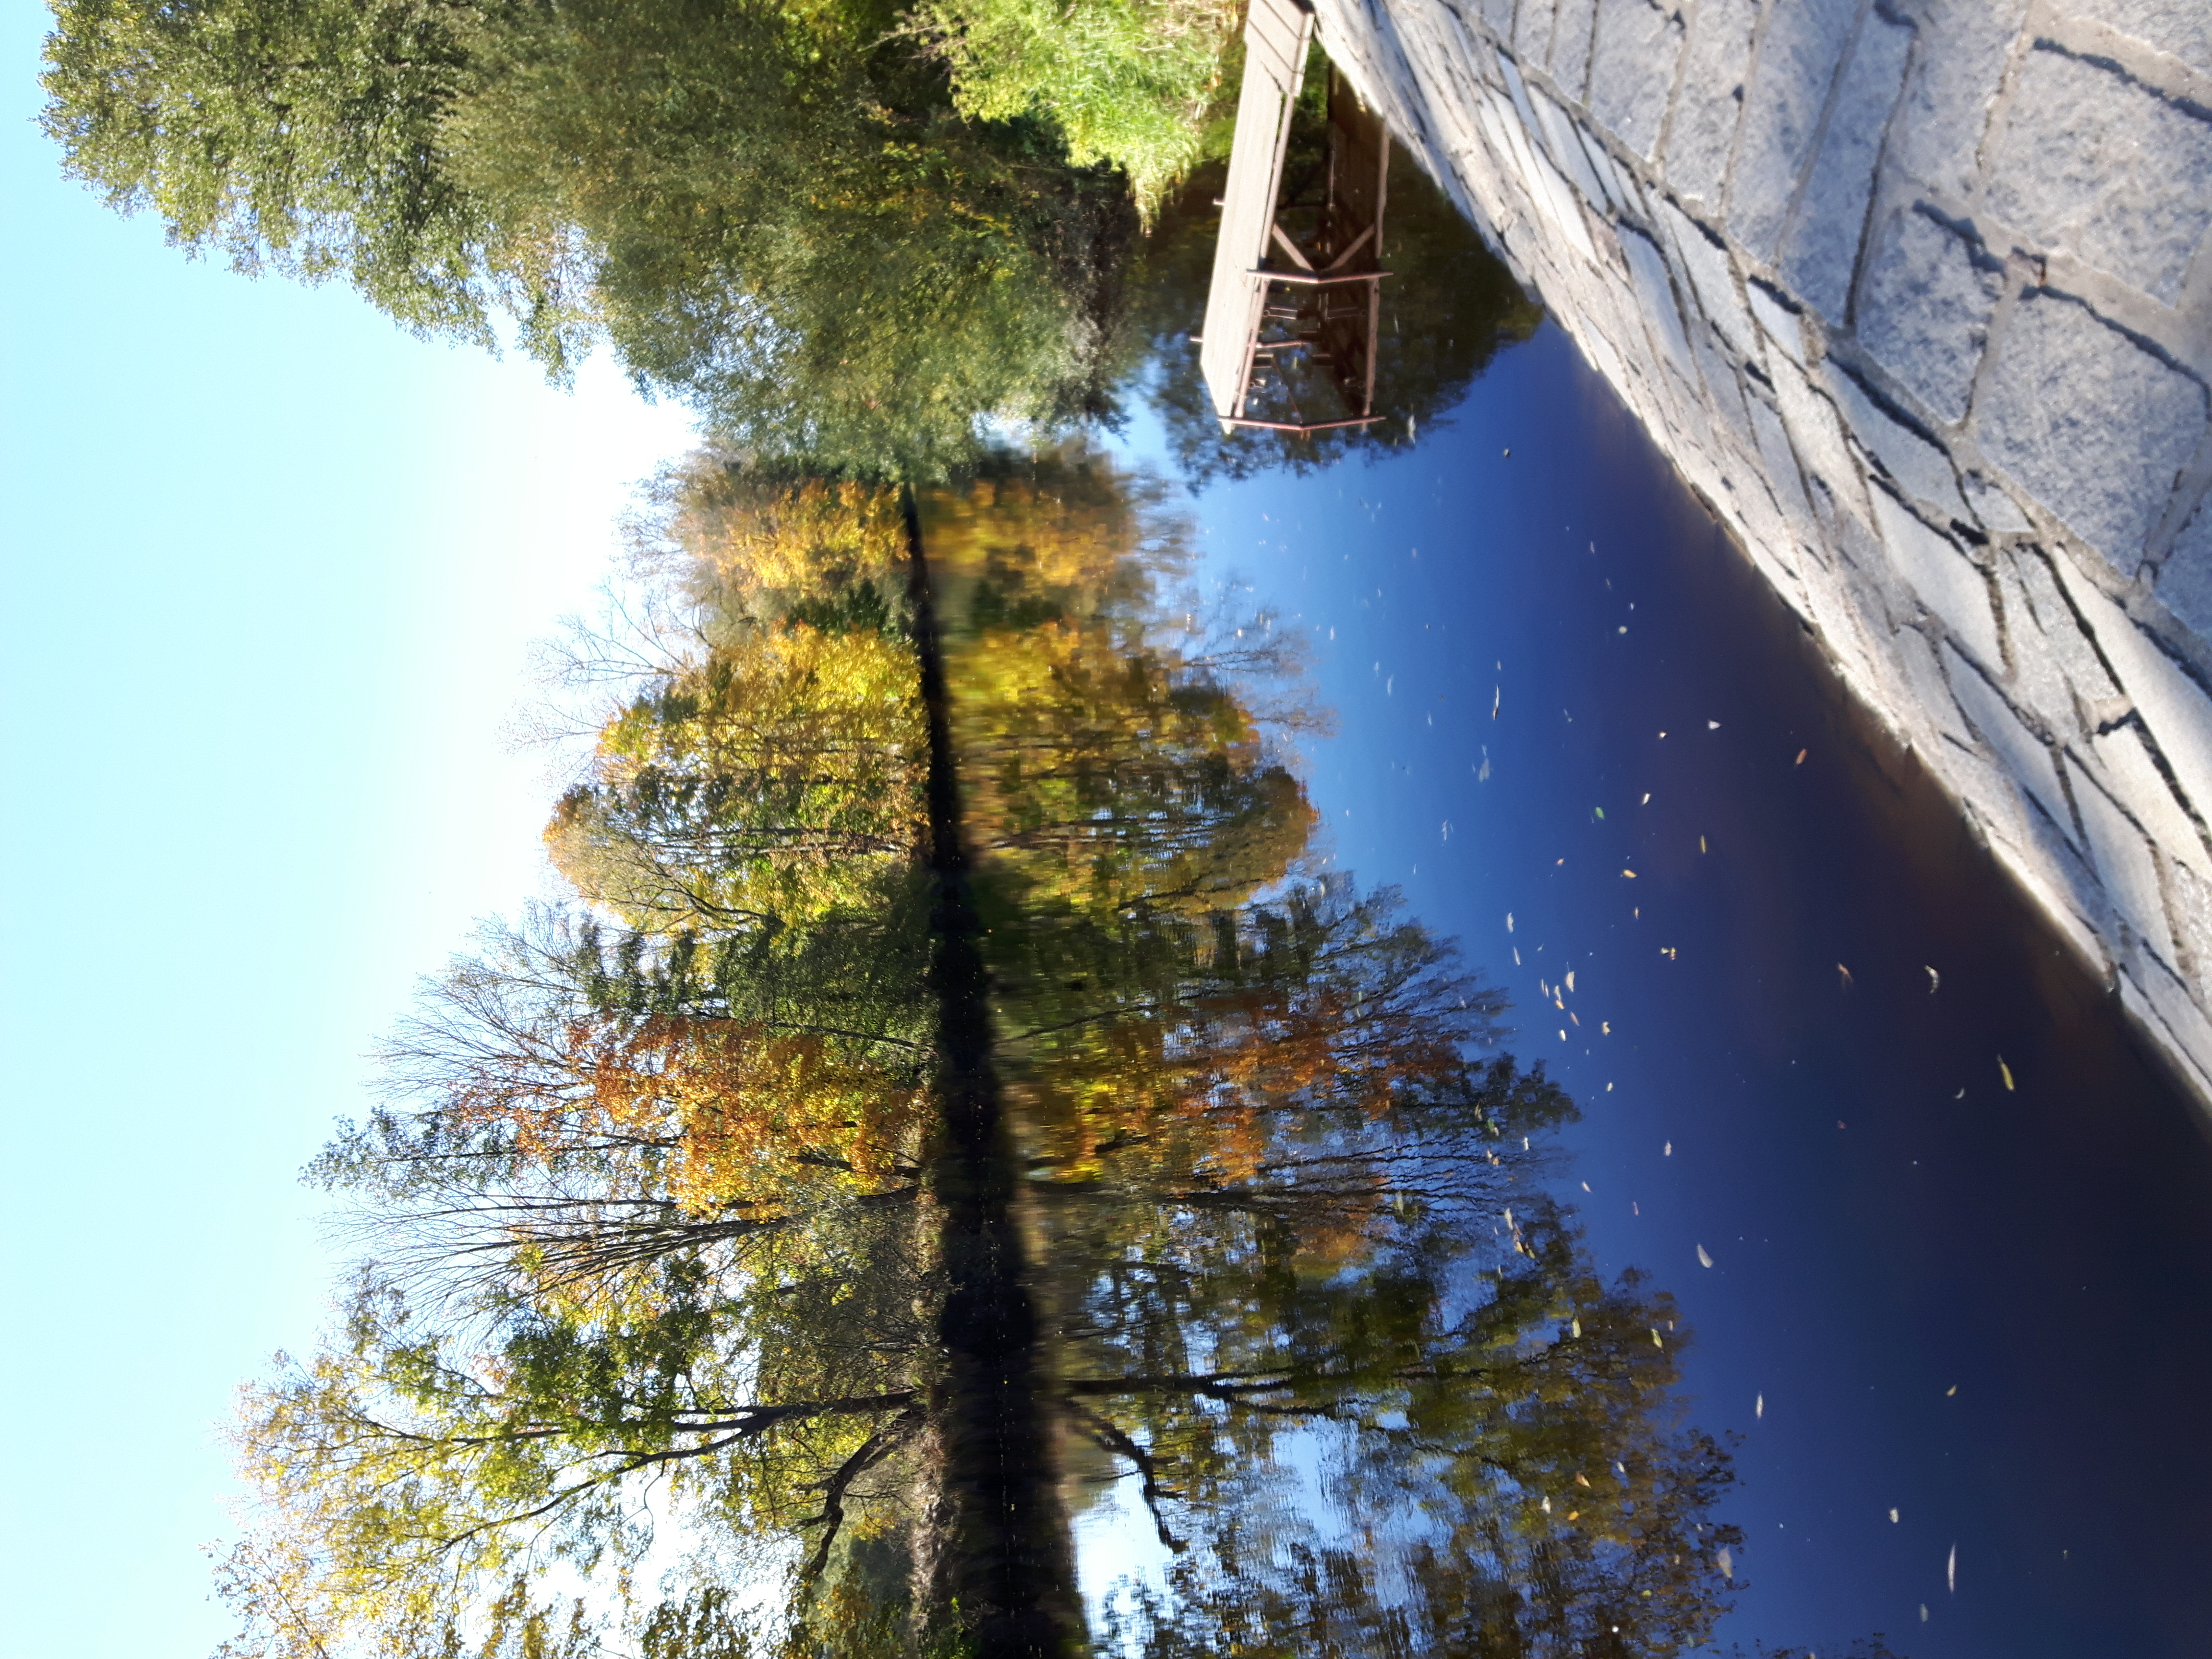
\includegraphics[width=11cm, angle =270]{pics/ot1.jpg}
	\caption{Otava na Podskalí ve Strakonicích na podzim}
	\label{obrazek:ot1}
\end{figure}


\subsection{Vysvětlení základních termínů}
Při hydrologické analýze je vhodná znalost základních pojmů. Ty jsou zde stručně popsány a vysvětleny, neboť jsou v rámci práce často používány. \cite{terminy}


\begin{description}
\item[Hustota říční sítě:] poměr délky všech toků k ploše povodí
\item[Povodí:] plocha území, ze kterého tok odvádí povrchovou a podpovrchovou vodu
\item[Pramen:] místo přirozeného výtoku podzemní vody, může být studený nebo termální, v oblastech se sopečnou činností gejzír
\item[Přítok:] tok nižšího řádu, který se vlévá do toku vyššího řádu
\item[Rozvodí:] hranice mezi jednotlivými povodími
\item[Rozvodnice:] pomyslná čára mezi sousedními povodími
\item[Říční síť:] půdorysná síť hlavního toku řeky a jejích přítoků, tvar je závislý na geologických a fyzickogeografických podmínkách povodí řeky
\item[Soutok:] místo, kde se setkávají nejméně dva vodní toky
\item[Úmoří:] plocha, ze které se všechna povrchová voda odvádí do moře nebo oceánu
\item[Ústí:] místo, kde se tok vlévá do jiného toku, vodní nádrže či oceánu
\item[Vodní tok:] voda tekoucí po zemském povrchu v korytě mezi břehy, větší toky jsou označovány jako řeky, menší toky jsou potoky
\item[Zátopové území:] část území v okolí vodních toků, které je periodicky zaplavované zvýšenými průtoky (pozn.: též inundace)
\end{description}



\subsection{Hydrologická analýza}
V rámci práce byla provedena jednoduchá základní hydrologická analýza. Pro~analýzu byla použita data z katalogu DIBAVOD. Pro tvorbu analýzy byl použit software ArcGIS a MS Excel. Analýza byla prováděna dle studijních materiálů Univerzity Karlovy Katedry fyzické geografie a geoekologie. \cite{UK}

Otava vzniká na Šumavě u Čeňkovy Pily soutokem Vydry a Křemelné. Vydra pramení na SZ svahu Luzného ve výšce 1215 m n. m. Díky okolním rašeliništím má Vydra rezavohnědou barvu. Svůj název si nese až po soutoku s Roklanským potokem v obci Modrava\footnote{V některých publikacích se uvádí název Vydra již od Březníku}. Řeka Křemelná pramení v Železnorudské hornatině v přírodní rezervaci Prameniště a severním svahu hory Pancíř (1214 m n. m.). \cite{SMOOS}

\begin{figure}[h!]
	\centering
	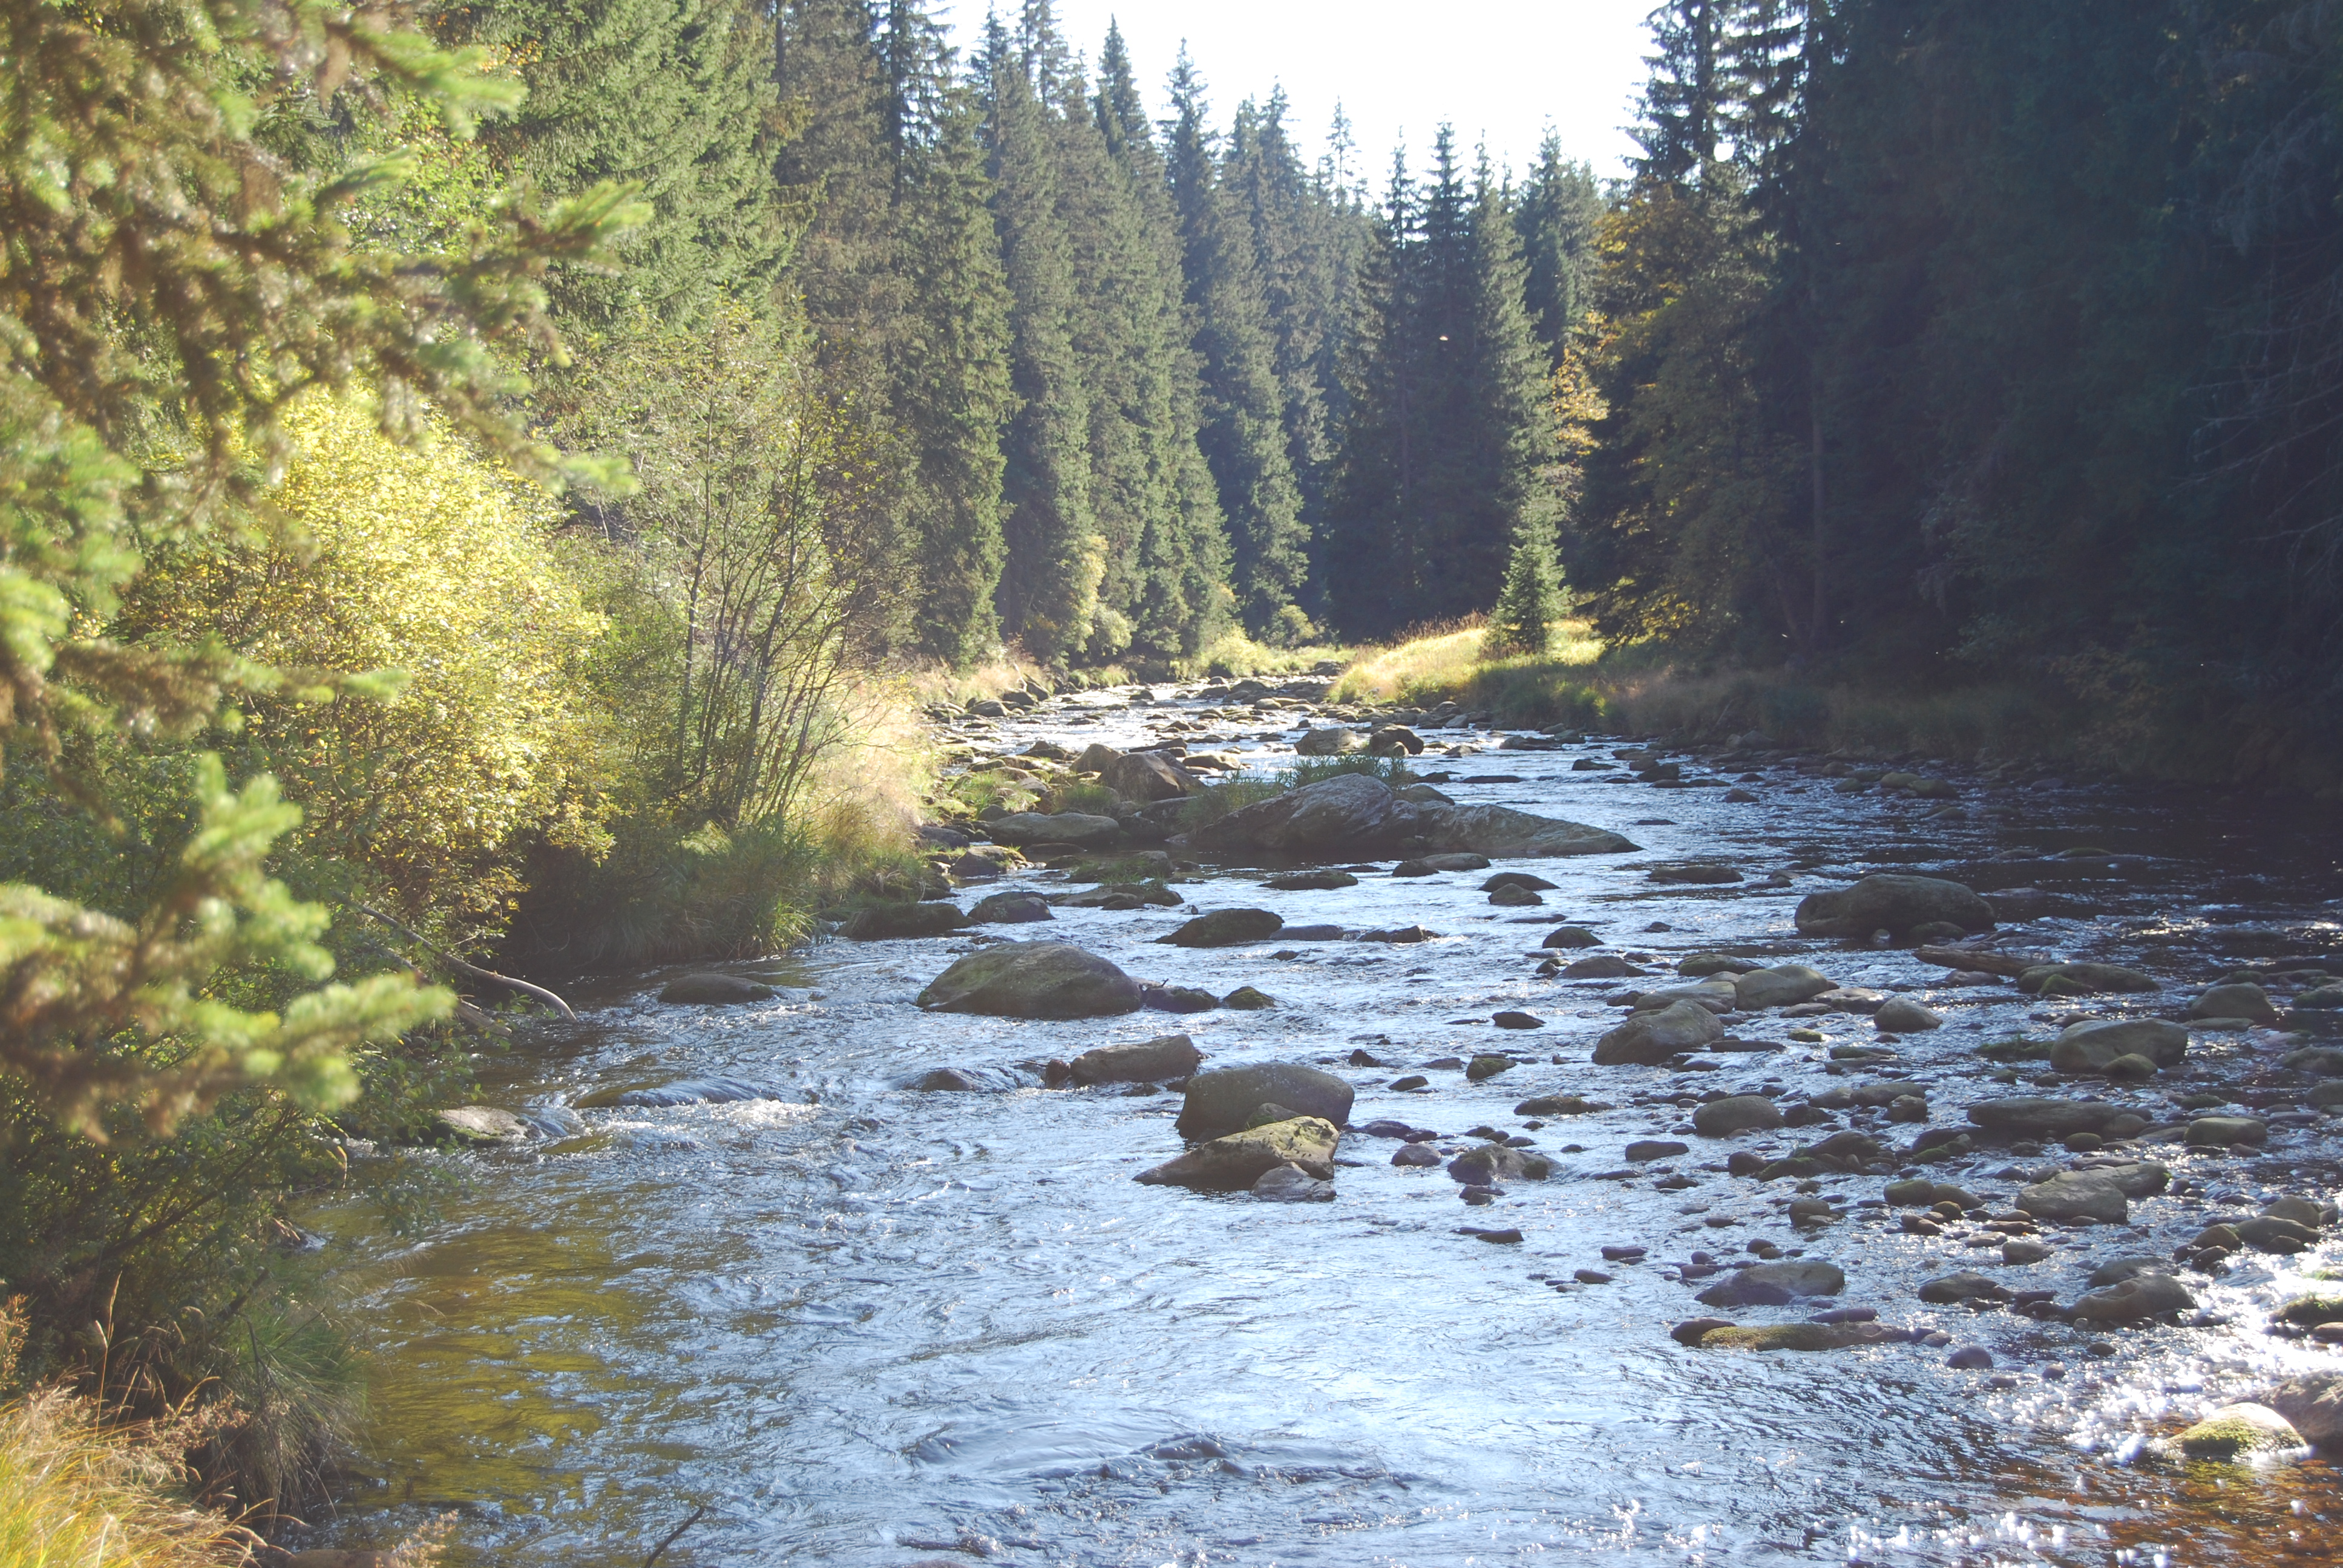
\includegraphics[width=12cm]{pics/vydra.jpg}
	\caption{Řeka Vydra}
	\label{obrazek:ot1}
\end{figure}

Řeka má několik přítoků. Mezi nejznámější patří řeka Ostružná, která ústí do Otavy nedaleko města Sušice. Významným přítokem je řeka Volyňka. Na~soutoku Volyňky a Otavy se nachází město Strakonice. Před Pískem do~Otavy vtéká Blanice. Poslední významnou řekou je Lomnice, která je levostranným přítokem Otavy. 

Otava je levostranným přítokem Vltavy, do níž se vlévá pod hradem Zvíkov poblíž Orlické přehrady. Povodí Otavy spadá do úmoří Severního moře (Otava~$\rightarrow$~Vltava~$\rightarrow$~Labe~$\rightarrow$~Severní moře ). 

Pokud bychom chtěli popsat řeku čísly, pak její délka je 111.7 km a plocha povodí 3841 km$^2$. Povodí Otavy lze označit jako vějířovité. 

\clearpage

\section{Významná města na Otavě}
Otava protéká několika historicky významnými městy. Mezi nejznámější města, kterými řeka protéká, patří Sušice, Horažďovice, Strakonice a Písek. Blíže popsány jsou také Žichovice z důvodu nedaleké zříceniny hradu Rabí.

\subsection{Sušice}
Sušice, označovaná také jako Brána Šumavy. Leží ve Svatoborské vrchovině na~řece Otavě. Název Sušice je pravděpodobně označení pro suché místo uprostřed vodních toků Otavy a Roušarky. Obydlení oblasti Sušice lze datovat na~přelom doby haltštatské a laténské v 5. století př. n. l. První obyvatelé byli Kelti, po nichž se do dneška dochovala dvě keltská hradiště, hradiště Sedlo, nacházející se zhruba 1 km jižně od Albrechtic, a Obří hrad, který lze nalézt přibližně 5 km jihovýchodně od Kašperských Hor. Hojné středověké osídlení bylo zapříčiněno množstvím zlata, které se v Sušici na Otavě rýžovalo. 

V polovině 13. století obsadil Sušicko Přemysl Otakar II. a z osady začal budovat královské město. Jan Lucemburský nechal v roce 1322 vybudovat městské hradby a potvrdil městu výsady královského města. Karel IV. utvrdil významnost města tím, že jej zařadil mezi města, jimž nesmí být zastavena nebo zcizena koruna. Sušice získala mílové právo a právo na vybírání mýtného. Běhěm husitských válek byla Sušice na straně husitů a měla velký podíl na~dobytí Švihova. 

\begin{figure}[h!]
	\centering
	\includegraphics[width=12cm]{pics/susice.jpg}
	\caption{Otava v Sušici s kaplí svatých Andělů Strážných v pozadí}
	\label{obrazek:susice}
\end{figure}

Během 16. století začala Sušice ztrácet na své významnosti. Zásoby zlata byly téměř vyčerpány a během 50 let došlo k šesti velkým požárům města. Za~vlády Ferdinanda I. navíc přišla Sušice z důvodu odepření pomoci o všechna svá privilegia a statky, navíc byla nucena odvádět dávky z piva a vína. Přesto měla Sušice velké příjmy z obchodu, neboť městem procházela Zlatá stezka, dříve nazývaná také jako "pasovská" či "solná". Vzhledem k této výhodné pozici si město vydobilo právo svobodného skladování soli. Během třicetileté války bylo město poničeno táhnoucími se vojsky a z důvodu rekatolizace se mnoho obyvatel rozhodlo odstěhovat. 

Po třicetileté válce byla vybudována poutní kaple svatých Andělů Strážných. Ve 2. polovině 17. století postihla Sušici morová epidemie, kvůli které byl vybudován nový hřbitov a kaple svatého Rocha. Během národního obrození vzniklo v Sušici ochotnické divadlo a rozvíjela se výuka českého jazyka. V roce 1839 byla založena společnost SOLO na výrobu zápalek. V roce 1933 byl zřízen podnik PAP vyrábějící obaly. 

V dnešní době se v Sušici nachází mnoho turisticky vyhledávaných míst. Na~vrcholu hory Svatobor se nachází kamenná vyhlídková věž,  v Muzeu Šumavy Sušice lze nalézt jeden z největších mechanických betlémů v České republice a od roku 2014 byl v Sušici obnoven pivovar, který vaří pivo Sušičák. \cite{SMOOS} \cite{susice}


\subsection{Žichovice}
Na soutoku Nezdického potoka a Otavy se nachází malebná obec Žichovice. První písemnou zmínku lze nalézt z roku 1045, kdy Břetislav I. věnoval Žichovice břevnovskému klášteru. Ve 2. polovině 16. století koupil Žichovice Jan Kavka Říčanský z Říčan a nechal zde vybudovat renesanční tvrz. Tvrz byla kolem roku 1603 přestavěna Janem Libštejnským z Kolovrat na renesanční zámek. Od roku 1964 je zámek chráněn jako kulturní památka. \cite{zichovice}

Žichovice se nachází zhruba 1 km jižně od zříceniny Rabí. Hrad byl založen rodem Wittelsbachů již v první polovině 13. století. S hradem se pojí mnoho pověstí, z nichž nejznámější je zřejmě pověst týkající se Jana Žižky, který zde údajně přišel o své druhé oko. Dohadů o ztrátě oka je však mnoho. Mezi~nejrozšířenější pověsti patří pověst o veliteli hradu Přibíku Kocovském, který z hradeb Rabí vystřelil šíp, kterým zasáhl právě oko Jana Žižky. Tento výjev byl poté zobrazen i na rabské bráně. Podle jiné pověsti se zabodl šíp do~hrušně, pod níž Žižka stál, a tříska ze stromu mu vypíchla oko. Po mnoho let se poté v oblasti Rabí chovala tradice vysazování hrušní. \cite{rabi}

Pro obec Žichovice měla Otava velký historický význam. V okolí se nachází stará rýžoviště zlata, je zde dlouhá vápenkářská tradice a bohatá historie voroplavby.

\begin{figure}[h!]
	\centering
	\includegraphics[width=12cm]{pics/zichovice.jpg}
	\caption{Žichovický jez, v pozadí zřícenina Rabí}
	\label{obrazek:zichovice}
\end{figure}

\subsection{Horažďovice}
Horažďovice leží v Horažďovické pahorkatině pod vrchem Prácheň. V roce 1293 byly Václavem II. povýšeny na město. Horažďovice, stejně jako Sušice a~Žichovice, byly využívány pro rýžování zlata a jako významný bod na obchodní stezce. O rozvoj města se nejvíce zasloužil rod Bavorů ze Strakonic. 

V Horažďovicích lze nalézt mnoho významných budov. Za zmínku stojí rozhodně zámecký komplex s panským pivovarem nacházející se na náměstí. V tomto zámku se nachází velký sál s freskovou výzdobou  (obrázek č. \ref{obrazek:hd}, zdroj \cite{hd}). Nástropní freska zachycuje bitvu husitů a císaře Zikmunda pod~Vyšehradem. Stěny sálu jsou pokryty výjevy z válek s Turky za vlády Leopolda I.  \cite{obce}\cite{hd}

\begin{figure}[h!]
	\centering
	\includegraphics[width=11cm]{pics/hd.jpg}
	\caption{Velký sál v Horažďovicích}
	\label{obrazek:hd}
\end{figure}



\subsection{Strakonice}
Strakonice, okresní město ležící v jižních Čechách na soutoku Otavy a Volyňky. Vzniklo spojením čtyř osad - Strakonic, Bezděkova, Lomu a Žabokrt. O~Strakonicích pochází první písemná zmínka z roku 1243, kdy Bavora I. se~svou manželkou Bolemilou věnuje okolní vsi, kostel a část hradu řádu johanitů. Ve~2. polovině 13. století nechává Bavor II. postavit hradní věž Rumpál, která stojí dodnes. 

\begin{figure}[h!]
	\centering
	\includegraphics[width=11cm]{pics/hrad.jpg}
	\caption{Pohled na Strakonický hrad ze západní strany}
	\label{obrazek:hrad}
\end{figure}

V roce 1367 bylo městu Bavorem IV. uděleno právo várečné. Pivo si vařili měšťané ve vlastních domech\footnote{Uvádí se, že v polovině 17. století se ve Strakonicích nacházelo až 158 domů s právem vařit pivo} a vrchnost v hradním pivovaru. V roce 1649 došlo k uskupení právovárečníků a byl založen měšťanský pivovar. Ten stojí ve~Strakonicích dodnes a je to poslední pivovar v České republice, který je ve~vlastnictví města. 

V roce 1357 postihl město velký požár, který zničil horní část města. Při~obnově bylo náměstí v této části rozšířeno, díky čemuž se protáhlo a mělo tvar dlouhého úzkého obdélníku. Obyvatele Strakonic dodnes tíží fakt, že místo náměstí mají spíše dlouhou ulici. Kromě požárů sužovaly město zejména povodně. Ty byly velmi časté a opakovaně zaplavovaly podhradí. Z toho důvodu neviděli Bavorové oblast Strakonicka za vhodnou pro založení města.

Během husitských válek byly Strakonice na straně katolického panstva a šlechtických rodů. Pro husitská vojska byl hrad nedobytný. Dobylo jej až během třicetileté války v roce 1619 císařské vojsko pod vedením Karla Longuevala. Město bylo drancováním švédskými vojsky natolik zdevastováno, že jej v roce 1645 velkopřevor Rudolf Colloredo z Wallsee osvobodil od placení válečných daní.

Po první světové válce byl hrad prodán agrárnímu sdružení a začal se ve~městě rozvíjet průmysl. Vznikla Jihočeská zbrojovka a ve velkém se ve~Strakonicích vyráběly turecké čepičky (fezy), které byly následně nahrazeny barety. 

Ze Strakonic pochází mnoho významných osobností, za zmínku určitě stojí František Ladislav Čelakovský, Josef Šmidinger, do Strakonic také zasadil svou báchorku o Strakonickém dudáku Josef Kajetán Tyl. Ve Strakonicích prožil své dětství Jiří Žáček a Josef Skupa a jednou z nejdůležitějších osobností byl Josef Režný, který založil Prácheňský soubor lidových písní a tanců (Prácheňáček) a byl spoluzakladatelem Jihočeské slavnosti písní a tanců, dnes nazvané Mezinárodní dudácký festival ve Strakonicích. \cite{obce}


\subsection{Písek}
Vznik Písku se datuje zhruba do poloviny 13. století. Město vzniklo v oblasti rýžoviště zlatého písku, z čehož lze usuzovat i původ jména města. V roce 1254 jej rozšířil Přemysl Otakar II. na královské město. Během 13. století vzniklo v Písku mnoho významných staveb: hrad, klášter, děkanský kostel, rychta a kamenný most, který je v současné době nejstarším kamenným mostem v~České republice. 

\begin{figure}[h!]
	\centering
	\includegraphics[width=11cm]{pics/pisek.jpg}
	\caption{Kamenný most v Písku}
	\label{obrazek:pisek}
\end{figure}

Písek byl ve 13. století jmenován na sídlo Prácheňského kraje. Během husitských válek bylo město centrem Jednoty táborské a Jan Žižka z Trocnova jej často navštěvoval. Za třicetileté války bylo město dobyto a vydrancováno. V 18. století se mu však opět vrátila všechna sláva a bohatství a v roce 1778 bylo v Písku otevřeno gymnázium. Písek bylo třetí české město, ve kterém bylo zřízeno elektrické osvětlení obloukovými lampami Františka Křižíka. Jedním z~nejznámějších obyvatel města je však Fráňa Šrámek, který Písek často používal jako dějiště svých děl. 

V současnosti je město jedním z vyhledávaných turistických cílů. Kromě zmíněného nejstaršího kamenného mostu se v Písku nachází několik kostelů a~kaplí, sladovna a Prácheňské muzeum.

\section{Významné skutečnosti související s Otavou}
\subsection{Rýžování zlata}
Hojné osídlení podél řeky Otavy bylo v minulosti dáno zejména četnými nálezy zlata v řece. Zlato se získávalo tzv. rýžováním. Při rýžování se do kovové pánve nabere směs písku z řeky a následnými krouživými pohyby na hladině jsou postupně lehké částice odplavovány a zlato zůstává na dně pánve. \cite{zlato}

Na Otavě se zlato rýžuje dodnes. V Kestřanech se koná každoročně soutěž v rýžování zlata, která probíhá v režii Českého klubu zlatokopů. 

\subsection{Voroplavba}
První zmínky o plavení dřeva na Otavě pochází již ze 14. století za doby vlády Jana Lucemburského. Šumavské dřevo bylo tehdy považováno za jeden z nejkvalitnějších stavebních materiálů a za vlády Karla IV. se nesmělo stavět z~jiných, než ze šumavských. Vysoká kvalita byla dána zejména tím, že vymáčené dřevo již nepracovalo a při vysoušení se nekroutilo a nepraskalo. 

V 19. století začala vznikat vaziště, ve kterých byly jednotlivé kusy dřeva vázány dohromady. Vaziště vzniklo např. v Dlouhé Vsi, v Žichovicích nebo v Katovicích. Vorařům se často přezdívalo "Hamburáci", neboť dřevo často plavili až do Hamburku. 

Po 2. světové válce začala významnost voroplavby upadat a při transportu se dávala přednost železniční a automobilové dopravě. V roce 1954 byla dokončena stavba vodní nádrže Slapy, která plavení dřeva definitivně ukončila. Paradoxně bylo dřevo pro tuto stavbu dopravováno po řece. Poslední vor na Otavě vyplul 12. září 1960. Historické fotografie a dokumenty zachycující voroplavbu jsou dodnes k vidění v Muzeu řeky Otavy a voroplavby ve Střelských Hošticích. 
\clearpage
\begin{figure}[h!]
	\centering
	\includegraphics[width=11cm]{pics/voroplavba.jpg}
	\caption{Voroplavba ve Strakonicích, 1920}
	\label{obrazek:voroplavba}
\end{figure}


\subsection{Povodeň v roce 2002}
V roce 2002 postihla Českou republiku silná povodeň. Byla to jedna z největších katastrof současnosti a mezi nejvíce postižené oblasti patřily jižní Čechy. Velké množství vody zatopilo téměř všechna města po proudu, v Písku povodeň dokonce poničila kamenný most. 

\begin{figure}[htp]
\centering
\includegraphics[width=6cm]{pics/povoden1.jpg}
\includegraphics[width=6cm]{pics/povoden1.jpg}
\caption{Povodeň v roce 2002 a aktuální stav}
\label{obr:povoden_hrad}
\end{figure}

\begin{figure}[h!]
\centering
\includegraphics[width=6cm]{pics/povoden2.jpg}
\includegraphics[width=6cm]{pics/povoden2.jpg}
\caption{Povodeň v roce 2002 a aktuální stav}
\label{obr:povoden_hrad}
\end{figure}

\begin{figure}[h!]
\centering
\includegraphics[width=6cm]{pics/povoden3.jpg}
\includegraphics[width=6cm]{pics/povoden3.jpg}
\caption{Povodeň v roce 2002 a aktuální stav}
\label{obr:povoden_hrad}
\end{figure}

\begin{figure}[h!]
\centering
\includegraphics[width=6cm]{pics/povoden4.jpg}
\includegraphics[width=6cm]{pics/povoden4.jpg}
\caption{Povodeň v roce 2002 a aktuální stav}
\label{obr:povoden_hrad}
\end{figure}

\chapter{Použitá data}
\section{Stavební plány Strakonického hradu}
Pro tvorbu 3D modelu Strakonického hradu byly použity stavební plány, které poskytl Stavební úřad ve Strakonicích. 

Stavební úřad měl k dispozici vypracované podklady získané Stavebně historickým průzkumem (SHP). SHP je metoda, která kompletně vypracuje a~zhodnotí historicky významnou stavební památku či historické jádro některých českých a moravských měst. Mezi prvními, kdo SHP prováděl, byl Kamil Hilbert na počátku 20. století. Následoval ho Oldřich Stefan z Ústavu dějin architektury ČVUT a doc. Václav Mencl z Filozofické fakulty Univerzity Karlovy. Po 2. světové válce bylo zdevastováno mnoho měst a významných památek. Z tohoto důvodu vznikl ústav R-ateliér, který rekonstruoval památky při organizaci Stavoprojekt. V roce 1954 byl R-ateliér přejmenován na Státní ústav pro rekonstrukce památkových měst a objektů (SÚRPMO). V SÚRPMO působilo několik významných osobností, za zmínku jistě stojí Dobroslav Líbal nebo Jan Muk. 

Mezi materiály, které měl k dispozici Stavební úřad ve Strakonicích, patří i vypracované podklady z SHP. Tyto materiály pochází ze 70. let 20. století a jsou v perfektním stavu a velmi detailně vypracovány. Na každém listu je ručně zakreslený erb Strakonic. Autor odvedl precizní a velmi kvalitní práci. Tyto materiály mají však v dnešní době vysokou hodnotu, tudíž nebylo možné je za účelem tvorby 3D modelu zapůjčit. Z tohoto důvodu byly použity plány vzniklé na počátku 21. století. \cite{shp}

\clearpage

\begin{figure}[h!]
	\centering
	\includegraphics[width=10cm]{pics/shp.jpg}
	\caption{Úvodní list materiálů ze stavebně historického průzkumu Strakonického hradu}
	\label{obrazek:shp}
\end{figure}


\section{Kartografické podklady}
\subsection{Císařské povinné otisky stabilního katastru}
Císařské povinné otisky stabilního katastru vznikaly na základě císařského patentu Františka I. z roku 1817. Aby byly mapy po celém území vyhotoveny stejným způsobem, byla v roce 1824 vydána měřická instrukce. Mapy vznikly za účelem přesného mapového podkladu pro stanovení pozemkové daně. Základní délkovou jednotkou byl Vídeňský sáh [$^\circ$] (1\,$^\circ$ = 1,896484 m).

Kartografické zobrazení těchto map bylo Cassini-Soldnerovo (transverzální válcové zobrazení). Kladná osa Y směřovala k západu a kladná osa X k~jihu. Jednalo se o zobrazení ekvidistantní v kartografických polednících, což znamená, že se vzdáleností od základního poledníku roste i veikost délkového zkreslení. Z tohoto důvodu bylo potřeba vytvořit několik soustav, pro Rakousko–Uhersko jich bylo použito 7. Při volbě soustav se vycházelo z požadavku na maximální zkreslení 50 cm/km. 

Na území Česka (nebo Československa??) byly použity tři soustavy. Jednalo se o soustavy s počátečním bodem Gusterberg (Horní Rakousy), sv. Štěpán (Vídeň) a Gellérthégy (Budapešť). V roce 1887 byla vydána nová měřická dokumentace, která již používala metrickou soustavu. Císařské povinné otisky byly původně uloženy v Centrálním archivu pozemkového katastru ve Vídni, po rozpadu Rakousko-Uherska byly převezeny do Prahy. Legendu těchto map můžete vidět na obrázku č. \ref{obrazek:legenda}. \cite{mapko}


\begin{figure}[h]
	\centering
	\includegraphics[width=13cm]{pics/legenda_CPO.png}
	\caption{Legenda císařských povinných otisků stabilního katastru}
	\label{obrazek:legenda}
\end{figure}

\subsection{Katastrální mapa}
Katastrální mapa je státní mapové dílo vydávané Českým úřadem zeměměřickým a katastrálním. Jedná se o mapy velkého měřítka (1 : 1000, 1 : 2880 apod.). Katastrální mapy jsou zpravidla vedeny v S-JTSK. Jejich hlavní využití je při zjišťování umístění pozemku v území a jako podklad pro územní a~stavební řízení, pro řízení o vyvlastnění pozemku apod. 

3 hlavní složky katastrální map jsou polohopis, popis a body. Polohopis obsahuje například hranice katastrálních území, státní hranice či hranice nemovitostí. Popis zahrnuje měřítko, označení sousedních mapových listů, označení parcel parcelními čísly nebo pomístní názvosloví\footnote{U digitálních map jsou mimorámové údaje obsaženy v metadatech}. Body jsou obsaženy pouze v~mapách, které jsou v S-JTSK a jedná se o body polohových bodových polí. \cite{cuzk}




\section{Fotodokumentace}
Součástí této práce je také vyhledání historických fotografií a jejich případné porovnání se současným stavem. Z historických fotografií byly použity fotografie ze sbírky Ladislava Hölla. Dále byly vyhledány fotografie na webových stránkách a 

\chapter{Příprava dat}

\section{Georeferencování}


\subsection{Transformace}
Co je transformace (versus projekce), využití atd)

\subsubsection{Obecná transformace}

\subsubsection{Transformace založené na vyrovnání MNČ}


\chapter{Zpracování dat}
\section{Tvorba 3D modelu Strakonického hradu}







\chapter{Prezentace na webových stránkách}


\chapter{Diskuze}



\begin{conclusion}
Závěr
\end{conclusion}

\bibliographystyle{csn690}
\bibliography{mybibliographyfile}

\appendix

\chapter{Seznam použitých zkratek}
% seřadit podle abecedy
% \printglossaries
\begin{description}
	\item[DIBAVOD] Digitální báze vodohospodářských dat
	\item[SHP] S

\end{description}



\chapter{Obsah přiloženého CD}

\begin{figure}
	\dirtree{%
		.1 readme.txt\DTcomment{stručný popis obsahu CD}.
		.1 grafy\DTcomment{složka obsahující výsledné grafy}.
		.1 rastry\DTcomment{složka obsahující testované rastry}.
		.1 rozklad.m\DTcomment{skript na výpočet rozkladu RGB barev}.
		.1 LaTex\DTcomment{zdrojová forma práce ve formátu \LaTeX{}}.	
		.1 text\DTcomment{text práce}.
		.2 BP\_Pasovska\_Petra\_2017\DTcomment{text práce v PDF}.	
	}
\end{figure}

\end{document}